% Replication presentation: Fajgelbaum et al. (2024), AER: Insights 6(2)
% STAT 5200 - Applied Econometrics I, Fall 2026
%
% Look: colours, slide title and footer copied from the Wharton PowerPoint
% template (Wharton_PPT_Template_16x9_v.3.1.pptx). Positions are the
% template's, scaled from its 33.87 x 19.05 cm slide to Beamer's 16 x 9 cm.
% The only other file the styling needs is graphics/WhartonLogoWhite.png.
%
% Layout rules used throughout:
%   - content starts at the top of every slide (class option t); blocks
%     that close a slide are pushed to the bottom with \framefill
%   - columns use [onlytextwidth], so they line up with the slide title
%   - full-width text is 11pt; text beside a figure is \small
%   - table numbers are aligned on the decimal point (column type d)

\documentclass[aspectratio=169,11pt,compress,t]{beamer}
\usepackage[utf8]{inputenc}
\usepackage[T1]{fontenc}
\usepackage{lmodern}               % LaTeX's own font (Latin Modern)
\usepackage{booktabs,graphicx,amsmath,tikz,dcolumn}
\usepackage[absolute,overlay]{textpos}

%%% ------------------------------------------------------------------
%%% Presenter notes
%%% ------------------------------------------------------------------
% Each frame ends with a \note{} holding a word-for-word script to read
% while recording (about 10 minutes, including short pauses between slides).
% The heading of each note gives the slide, how long to spend on it and
% the clock time at which it should end; paragraph breaks mark pauses.
%
% To get the notes, change \shownotesfalse to \shownotestrue and compile:
% each page of the PDF is then twice as wide, with the slide on the left
% and its notes on the right. A presenter app such as pympress splits these
% pages into a slide window (to share in Zoom) and a notes window.
% Change it back to compile the slides on their own.
\newif\ifshownotes
\shownotesfalse
\ifshownotes\setbeameroption{show notes on second screen=right}\fi

%%% ------------------------------------------------------------------
%%% Wharton look
%%% ------------------------------------------------------------------
% Template colour scheme
\definecolor{PennNavy}{HTML}{011F5B}     % accent 1, body text, footer band
\definecolor{PennRed}{HTML}{C5093B}      % slide titles, footer slash
\definecolor{PennDarkRed}{HTML}{990000}  % accent 2
\definecolor{PennBlue}{HTML}{026CB5}     % accent 3
\definecolor{PennSky}{HTML}{06AAFC}      % accent 4
\definecolor{PennLight}{HTML}{EEEDEA}    % light background
\definecolor{FooterGray}{HTML}{AFAFAF}   % footer text and slide number

\setbeamercolor{normal text}{fg=PennNavy}
\setbeamercolor{structure}{fg=PennNavy}
\setbeamercolor{frametitle}{fg=PennRed}
\setbeamercolor{alerted text}{fg=PennRed}
\setbeamercolor{section number projected}{bg=PennNavy,fg=white}
\setbeamercolor{block title}{bg=PennNavy,fg=white}
\setbeamercolor{block body}{bg=PennLight,fg=PennNavy}
\setbeamercolor{block title alerted}{bg=PennDarkRed,fg=white}
\setbeamercolor{block body alerted}{bg=PennLight,fg=PennNavy}

% Fonts: Beamer's default LaTeX font throughout
\setbeamerfont{frametitle}{size=\fontsize{14}{16}}
\setbeamerfont{block title}{series=\bfseries,size=\small}
\setbeamerfont{block body}{size=\small}

% Margins as in the template (title and body start 1.1 cm from the left)
\setbeamersize{text margin left=1.1cm,text margin right=1.1cm}

\setbeamertemplate{navigation symbols}{}
\setbeamertemplate{blocks}[default]
\setbeamertemplate{section in toc}[ball numbered]

% Bullets: red dot for the first level, blue dash for the second
\setbeamertemplate{itemize item}{\color{PennRed}\raisebox{0.1ex}{\small$\bullet$}}
\setbeamertemplate{itemize subitem}{\color{PennBlue}\raisebox{0.1ex}{\footnotesize\textendash}}

% Spacing: some air between first-level points, tighter second level.
% A 16:9 Beamer slide is only 9 cm tall, and the navigation bar, slide
% title and footer take about 2.3 cm of it, leaving about 6.7 cm (190pt)
% for content. Every slide below is budgeted to stay under about 170pt.
\addtobeamertemplate{itemize/enumerate body begin}{}{\setlength{\itemsep}{0.35em}}
\addtobeamertemplate{itemize/enumerate subbody begin}{}{%
  \setlength{\itemsep}{0.05em}\vspace{0.05em}}

% Navigation bar: navy band across the top, matching the footer. Each
% section's (short) name with one circle per slide below it; the current
% slide's circle is filled and the other sections are dimmed. The circles
% are links. Sections use their short names: \section[short]{long}.
\setbeamercolor{section in head/foot}{fg=white,bg=PennNavy}
\setbeamercolor{mini frame}{fg=white}
\setbeamerfont{section in head/foot}{size=\fontsize{6}{7}}
\setbeamertemplate{mini frames}[default]
\setbeamertemplate{headline}{%
  \begin{beamercolorbox}[wd=\paperwidth]{section in head/foot}
    \vskip3pt\insertnavigation{\paperwidth}\vskip3pt
  \end{beamercolorbox}%
}

% Slide title: red text on white, top left, below the navigation bar.
% Beamer already places the title inside the 1.1 cm text margin, so no
% extra indent here: the title lines up with the text below it.
\setbeamertemplate{frametitle}{%
  \vspace*{0.15cm}%
  \parbox[t]{\textwidth}{\raggedright
    \usebeamercolor[fg]{frametitle}\usebeamerfont{frametitle}%
    \strut\insertframetitle\strut}\par
  \vspace*{0.1cm}%
}

% Footer: navy band across the bottom; white logo on the left;
% short title, red slash and bold slide number in grey on the right
\setbeamertemplate{footline}{%
  \begin{tikzpicture}
    \useasboundingbox (0,0) rectangle (\paperwidth,0.505cm);
    \fill[PennNavy] (0,0) rectangle (\paperwidth,0.505cm);
    \node[anchor=west,inner sep=0pt] at (0.2cm,0.2525cm)
      {
\includegraphics[height=0.227cm]{graphics/WhartonLogoWhite}};
    \node[anchor=east,inner sep=0pt,text=FooterGray,
          font=\fontsize{6}{7}\selectfont] at (14.97cm,0.2525cm)
      {\insertshorttitle};
    \draw[PennRed,line width=0.9pt] (15.21cm,0.125cm) -- (15.34cm,0.40cm);
    \node[anchor=east,inner sep=0pt,text=FooterGray,
          font=\fontsize{6}{7}\selectfont\bfseries] at (15.68cm,0.2525cm)
      {\insertframenumber};
  \end{tikzpicture}%
}

% Title slide (navy background, set on the frame below): white logo
% top left, white bold title, subtitle, author and date in light blue
\setbeamertemplate{title page}{%
  \begin{textblock*}{4.8cm}(0.76cm,0.70cm)
    
\includegraphics[width=4.8cm]{graphics/WhartonLogoWhite}
  \end{textblock*}
  \begin{textblock*}{13.3cm}(0.76cm,4.2cm)
    \raggedright
    {\color{white}\fontsize{18}{21}\selectfont\bfseries\inserttitle\par}
    \vspace{0.25cm}
    {\color{white}\fontsize{11}{13}\selectfont\insertsubtitle\par}
    \vspace{0.5cm}
    {\color{PennSky}\fontsize{9}{11}\selectfont\insertauthor\par\insertdate\par}
  \end{textblock*}
}

% Notes page: slide heading and timing in red, then the script, large
% enough to read from the screen. Text in grey brackets is a cue only.
\setbeamertemplate{note page}{%
  \vspace*{0.35cm}%
  \begin{minipage}[t]{\dimexpr\paperwidth-2.0cm\relax}
    \usebeamercolor[fg]{normal text}\small\raggedright
    \insertnote
  \end{minipage}}
% \notehead{slide}{time on slide}{ends at}
\newcommand{\notehead}[3]{%
  {\color{PennRed}\bfseries #1\hfill #2\enspace\textbar\enspace ends at #3}%
  \\[-0.2em]{\color{PennRed}\rule{\linewidth}{0.5pt}}\\[0.3em]}
% A stage direction in the notes, not read out
\newcommand{\cue}[1]{{\color{gray}\itshape [#1]}}

%%% ------------------------------------------------------------------
%%% Layout helpers
%%% ------------------------------------------------------------------
% Outline: the sections, numbered and starting at the left margin, in
% line with the slide title. \sectionoutline{n} prints section n in bold red and
% dims the others (the slide shown when a new section starts);
% \sectionoutline{0} prints them all alike (the outline slide).
\newcommand{\outlineitem}[3]{%
  \ifnum#1=0 {#2.\enspace #3}%
  \else\ifnum#1=#2 {\color{PennRed}\bfseries #2.\enspace #3}%
  \else {\color{PennNavy!40}#2.\enspace #3}\fi\fi\par\vspace{0.9em}}
\newcommand{\sectionoutline}[1]{{\large
  \outlineitem{#1}{1}{The question and the data}
  \outlineitem{#1}{2}{Replication: average export responses}
  \outlineitem{#1}{3}{The rest of the paper}
  \outlineitem{#1}{4}{Takeaways}}}

% Push what follows to the bottom of the slide
\newcommand{\framefill}{\vskip0pt plus 1filll}

% Heading over a column of bullets: bold, with a thin rule underneath
\newcommand{\colhead}[1]{%
  {\bfseries #1\par}\vspace{1pt}%
  {\color{PennNavy!25}\rule{\linewidth}{0.6pt}\par}\vspace{-0.2em}}

% Label over a figure ("Paper", "Replication")
\newcommand{\figlabel}[1]{{\footnotesize\bfseries #1\par}\vspace{3pt}}

% Table column aligned on the decimal point and centred on it
\newcolumntype{d}{D{.}{.}{-1}}
% Header cell in a d column
\newcommand{\hd}[1]{\multicolumn{1}{c}{#1}}

% A replicated number that differs from the paper, shown in red. In a d
% column the integer and decimal parts are coloured separately:
% \df{0}{22^{***}} prints 0.22***, \df{-3}{00} prints -3.00.
\newcommand{\df}[2]{\textcolor{PennRed}{#1}.\textcolor{PennRed}{#2}}

% Post-period slopes beside a figure: \slopes{title}{table rows}. The
% column is only 3.9 cm wide, so each value is a number (right-aligned)
% followed by its stars: \pv{0.31}{***} for a value, \pr{0.22}{***} for
% one that differs from the paper (red).
\newcommand{\pv}[2]{#1 & $^{#2}$}
\newcommand{\pr}[2]{\textcolor{PennRed}{#1} & \textcolor{PennRed}{$^{#2}$}}
\newcommand{\slopes}[2]{%
  {\footnotesize\bfseries #1\par}\vspace{3pt}%
  {\footnotesize\setlength{\tabcolsep}{3pt}%
  \begin{tabular}{@{}l r@{}l r@{}l@{}}
  \toprule
  Panel & \multicolumn{2}{c}{Paper} & \multicolumn{2}{c}{Repl.} \\
  \midrule
  #2
  \bottomrule
  \end{tabular}\par}%
  \vspace{2pt}{\scriptsize\textcolor{PennRed}{Red}: differs from the paper\par}}

% Figures: the paper's (authors' replication package, openICPSR E194689V1)
% and ours (Replication Study/Figures, copied here so the folder compiles
% on its own; copy them again after re-running didplots.py). Named by the
% paper's numbering: A.3 is US-China bilateral trade, A.4 adds exporter x
% sector fixed effects.
\newcommand{\figh}{5.2cm}    % height of the portrait figures

%%% ------------------------------------------------------------------

\title[Replication: Fajgelbaum et al.\ (2024)]{The US--China Trade War and
  Global Reallocations}
\subtitle{A replication of Fajgelbaum, Goldberg, Kennedy, Khandelwal \&
  Taglioni, \textit{AER: Insights} (2024)}
\author[Apostolos Kyratzis]{Apostolos Kyratzis - 13130833}
\date{STAT 5200 -- Applied Econometrics I, Fall 2026}

\begin{document}

{\setbeamercolor{background canvas}{bg=PennNavy}
\begin{frame}[plain]
\titlepage
\note{\notehead{1. Title}{0:15}{0:15}
  Hello, I'm Apostolos Kyratzis. I'll present my replication of Fajgelbaum and coauthors' paper, ``The US--China Trade War and Global Reallocations,'' published in AER: Insights in 2024.}
\end{frame}}

\begin{frame}[c]{Outline}
\sectionoutline{0}
\note{\notehead{2. Outline}{0:10}{0:25}
  I'll introduce the question and data, explain the replication results, briefly cover the rest of the paper, and finish with the takeaways.}
\end{frame}

%%% ==================================================================
\section[1. Question \& data]{The question and the data}
%%% ==================================================================

\begin{frame}{Did the trade war only reshuffle trade?}
\begin{itemize}
  \item 2018--19: the US and China tax each other's goods, about \$450bn
        of trade
  \item What happened to the \textbf{bystanders}, the other exporters?
  \begin{itemize}
    \item \emph{Reallocation}: exports diverted to the US and China, away
          from RW
    \item \emph{Expansion}: tariff-exposed exports rise across markets
  \end{itemize}
  \item Paper: stronger relative export growth to the US and RW;
        no detectable average response into China
\end{itemize}
\framefill
\begin{block}{This replication}
Section III, the average export responses: Figure 1, Table A.2 and
Figures A.3--A.4, rebuilt from raw data in Python
\end{block}
\note{\notehead{3. Did the trade war only reshuffle trade?}{0:50}{1:15}
  In 2018 and 2019, the US and China raised tariffs on each other's goods, covering roughly 450 billion dollars of trade. The authors ask what happened to other exporters, which they call bystanders.
\\[0.6em]
  These countries could redirect exports toward the US and China, reducing sales elsewhere. Alternatively, they could expand exports across markets.
\\[0.6em]
  The paper finds stronger export growth to the US and the rest of the world in tariff-exposed products, with no detectable average response into China. My replication covers these average responses: Figure 1, Table A.2, and the two appendix figures, using Python to rebuild the analysis from raw inputs.}
\end{frame}

\begin{frame}{Data}
\begin{columns}[T,onlytextwidth]
  \begin{column}{0.47\textwidth}
    \colhead{Trade flows}
    \small
    \begin{itemize}
      \item UN Comtrade ``Plus'' bulk files, HS 2012, 2014--19
      \item Totals over customs procedures and transport modes; US\$
            millions
      \item Exports measured from the importers' records
      \item Top 50 exporters selected after excluding oil exporters
    \end{itemize}
  \end{column}
  \begin{column}{0.47\textwidth}
    \colhead{Tariffs}
    \small
    \begin{itemize}
      \item \textbf{US on China}: HS10 tariffs from the US Census imports,
            weighted to HS6 by 2015--17 trade with China
      \item \textbf{China on US}: HS8 retaliation lists, 2019 exemptions
            (Bown et al.), weighted by China's 2017 imports from the US
      \item Measured as the change in $\log(1+\text{tariff})$
    \end{itemize}
  \end{column}
\end{columns}
\note{\notehead{4. Data}{0:50}{2:05}
  The left column describes the trade data. I use UN Comtrade bulk files for 2014 through 2019, with products classified at six digits. I retain total trade across customs procedures and transport modes, measured in millions of dollars. Exports are recorded using the importing country's reports, and the sample selects fifty major exporters after excluding oil exporters.
\\[0.6em]
  On the right are the tariff inputs. US tariffs come from the authors' Census import file, weighted using 2015--17 trade with China. Chinese tariffs come from retaliation lists and exemptions, weighted using China's 2017 imports from the US. Both are aggregated to six-digit products. Tariff changes are measured in log one plus the tariff rate.}
\end{frame}

\begin{frame}{Specification}
\vspace{-0.6em}
\[
  \Delta \ln X^{n}_{i\omega} \;=\; \alpha \;+\; \beta\, \Delta \ln T_{\omega}
  \;+\; \varepsilon_{i\omega}
\]
\vspace{-0.8em}
\begin{itemize}
  \item Outcome: log change in $i$'s exports of $\omega$ to
        $n \in \{\text{US}, \text{CH}, \text{RW}\}$
        (\texttt{dlv\_us}, \texttt{dlv\_ch}, \texttt{dlv\_rw})
  \item Tariff: change in $\log T$, where $T=1+t$ and $t$ is the tariff
        rate; US on CH (\texttt{dlz\_usch}) or CH on US (\texttt{dlz\_chus})
  \item Periods 2014/15, 2016/17, 2018/19: \textbf{post} 2017$\to$19,
        \textbf{pre} 2015$\to$17 with the war-period tariff change
        (a placebo)
  \item OLS, clustered by HS6; robustness with exporter $\times$ sector
        fixed effects
\end{itemize}
\note{\notehead{5. Specification}{0:55}{3:00}
  The equation relates export-value growth to the tariff increase imposed on a competing supplier. A positive beta means bystander exports grew faster in products facing larger tariffs on US or Chinese goods.
\\[0.6em]
  I estimate separate relationships for exports to the US, China, and the rest of the world, abbreviated RW.
\\[0.6em]
  The year labels represent two-year totals. The war-period comparison is 2016--17 against 2018--19. The prewar comparison uses 2014--15 against 2016--17, but keeps the same subsequent tariff changes. This checks whether the later-targeted products were already on different trends.
\\[0.6em]
  Estimation is by ordinary least squares, with standard errors clustered by product. The robustness specification adds exporter-by-sector fixed effects.}
\end{frame}


\begin{frame}{The replication pipeline}
\centering\footnotesize
\begin{tabular}{@{}l l p{8.1cm}@{}}
\toprule
Step & Script & Output \\
\midrule
Download   & \texttt{comtrade\_download.py} & 957 Comtrade files (14.6\,GB), logged with SHA-256 \\
Weights    & \texttt{china\_weight.py}      & HS10 shares of 2015--17 US--China trade in each HS6 \\
US tariffs & \texttt{z\_usch.py}            & US tariffs on China, by HS6 and period \\
CH tariffs & \texttt{z\_chus.py}            & China's tariffs on the US, by HS6 and period \\
Trade      & \texttt{comtrade.py}           & Bilateral trade by HS6, one file per year \\
Panel      & \texttt{build.py}              & \texttt{data5}: exporter $\times$ HS6 $\times$ period, top 50 exporters \\
Analysis   & \texttt{didplots.py}           & 20 regressions; Figures 1, A.3, A.4; Table A.2 \\
\bottomrule
\end{tabular}
\framefill
\raggedright
\begin{block}{Stata $\to$ Python}
Steps 2--7 port do-files: \texttt{reghdfe} becomes OLS with clustered
errors (FE: singletons dropped, same small-sample correction).
\end{block}
\note{\notehead{6. The replication pipeline}{0:30}{3:30}
  This table follows the replication from inputs to results. I downloaded 957 Comtrade files, built the trade weights and both tariff series, processed the bilateral flows, and assembled the exporter-product panel. The final script produces twenty regressions and the figures and table.
\\[0.6em]
  The processing and analysis translate the authors' Stata code into Python, matching their treatment of fixed effects and clustered standard errors.}
\end{frame}

%%% ==================================================================
\section[2. Replication]{Replication: average export responses}
%%% ==================================================================

\begin{frame}[c]{Outline}
\sectionoutline{2}
\note{\notehead{7. Outline: section 2}{0:05}{3:35}
  I'll now compare the replicated results with the paper.}
\end{frame}

\begin{frame}{Figure 1: paper vs.\ replication}
\begin{columns}[T,onlytextwidth]
  \begin{column}{0.335\textwidth}
    \centering
    \figlabel{Paper}
    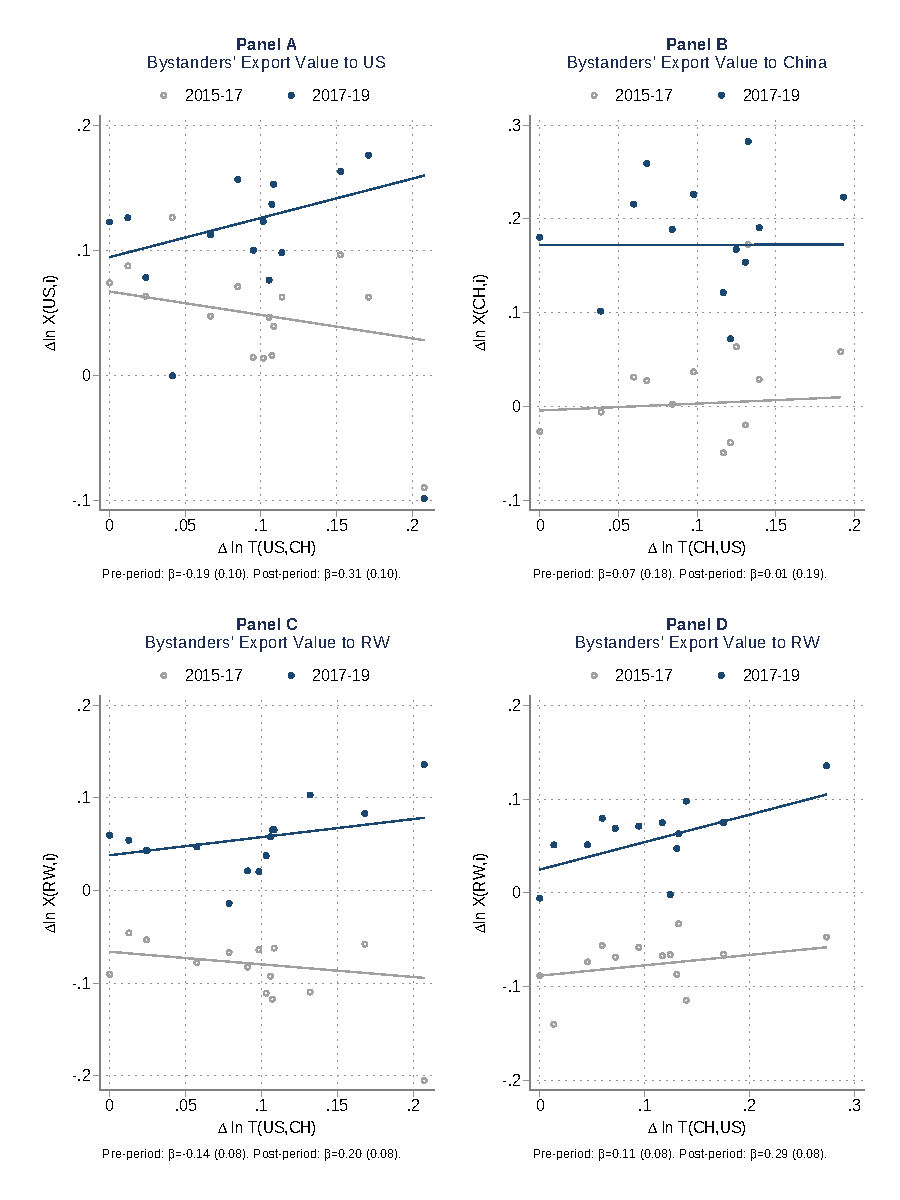
\includegraphics[width=\linewidth,height=\figh,keepaspectratio]{figures/paper/fig_1.pdf}
  \end{column}
  \begin{column}{0.335\textwidth}
    \centering
    \figlabel{Replication}
    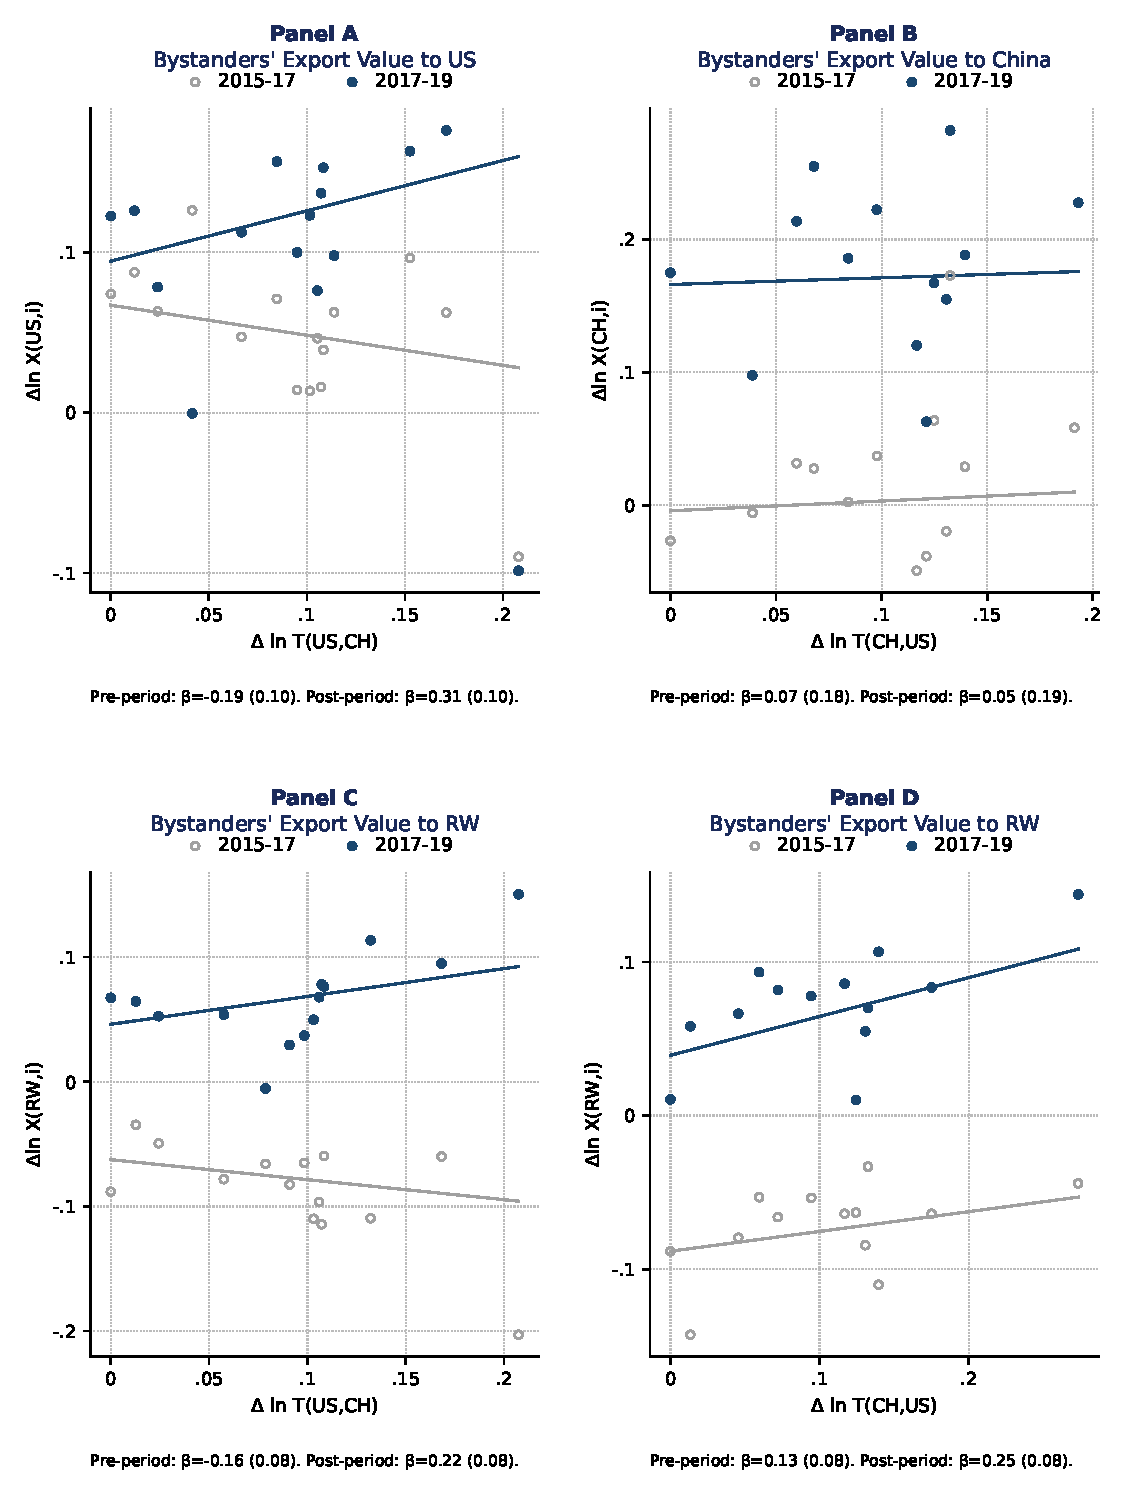
\includegraphics[width=\linewidth,height=\figh,keepaspectratio]{figures/replication/fig_1.pdf}
  \end{column}
  \begin{column}{0.28\textwidth}
    \slopes{Post-period slope, 2017--19}{%
      A\enspace US & \pv{0.31}{***} & \pv{0.31}{***} \\
      B\enspace CH & \pv{0.01}{} & \pr{0.05}{} \\
      C\enspace RW & \pv{0.20}{***} & \pr{0.22}{***} \\
      D\enspace RW & \pv{0.29}{***} & \pr{0.25}{***} \\}
    \vspace{0.5em}
    {\footnotesize\raggedright Panel A identical; B--D within 0.05\par}
  \end{column}
\end{columns}
\note{\notehead{8. Figure 1: paper vs.\ replication}{1:15}{4:50}
  The paper's Figure 1 is on the left, my replication is in the middle, and the postwar slopes are on the right.
\\[0.6em]
  The horizontal axis measures tariff changes; the vertical axis measures bystanders' export-value growth. Each dot averages observations within a tariff bin. Blue represents the war period; grey represents prewar growth against the same later tariff changes.
\\[0.6em]
  In Panel A, US tariffs on China are associated with stronger bystander exports to the US. Panel B shows no statistically detectable average response into China.
\\[0.6em]
  Panels C and D show that exports to the rest of the world also grew faster in products facing higher US or Chinese tariffs. That is the important distinction from simply redirecting exports toward the US.
\\[0.6em]
  The estimates are close: Panel A is 0.31 in both versions. My China estimate is 0.05, while the rest-of-world estimates are 0.22 and 0.25. Each differs from the paper by less than 0.05.}
\end{frame}

\begin{frame}{Table A.2: coefficients}
\centering\small
\begin{tabular}{@{}ll dd dd@{}}
\toprule
 & & \multicolumn{2}{c}{Post: 2017--19} & \multicolumn{2}{c}{Pre: 2015--17} \\
\cmidrule(lr){3-4}\cmidrule(l){5-6}
Exports to & Tariff & \hd{Paper} & \hd{Replication} & \hd{Paper} & \hd{Replication} \\
\midrule
US & US on CH & 0.31^{***} & 0.31^{***}       & -0.19^{*} & -0.19^{*} \\
   &          & (0.10)     & (0.10)           & (0.10)    & (0.10) \\
CH & CH on US & 0.01       & \df{0}{05}       & 0.07      & 0.07 \\
   &          & (0.19)     & (0.19)           & (0.18)    & (0.18) \\
RW & US on CH & 0.20^{***} & \df{0}{22^{***}} & -0.14^{*} & \df{-0}{16^{**}} \\
   &          & (0.08)     & (0.08)           & (0.08)    & (0.08) \\
RW & CH on US & 0.29^{***} & \df{0}{25^{***}} & 0.11      & \df{0}{13^{*}} \\
   &          & (0.08)     & (0.08)           & (0.08)    & (0.08) \\
\bottomrule
\end{tabular}

\vspace{2pt}
{\scriptsize Clustered s.e.\ in parentheses;
$^{*}p<0.10$, $^{**}p<0.05$, $^{***}p<0.01$;
\textcolor{PennRed}{red}: differs from the paper.\\
Post-period $N$, paper: 102{,}903; 90{,}128; 223{,}556; 223{,}556.
Replication: 102{,}903; 90{,}100; 223{,}903; 223{,}903.\par}
\note{\notehead{9. Table A.2: coefficients}{0:45}{5:35}
  This table reports the coefficients and standard errors behind those lines. The left pair of columns covers the war period; the right pair covers the prewar comparison. Red identifies differences from the paper.
\\[0.6em]
  For exports to the US, the slope is 0.31. A ten-log-point increase in the tariff factor is therefore associated with roughly three percent faster export growth.
\\[0.6em]
  The postwar signs and significance levels match the paper. Standard errors also match at two decimal places, and sample sizes are very close. Two rest-of-world prewar estimates become more significant; I'll return to that caveat.}
\end{frame}

\begin{frame}{Robustness: exporter $\times$ sector FE (Fig.\ A.4)}
\begin{columns}[T,onlytextwidth]
  \begin{column}{0.335\textwidth}
    \centering
    \figlabel{Paper}
    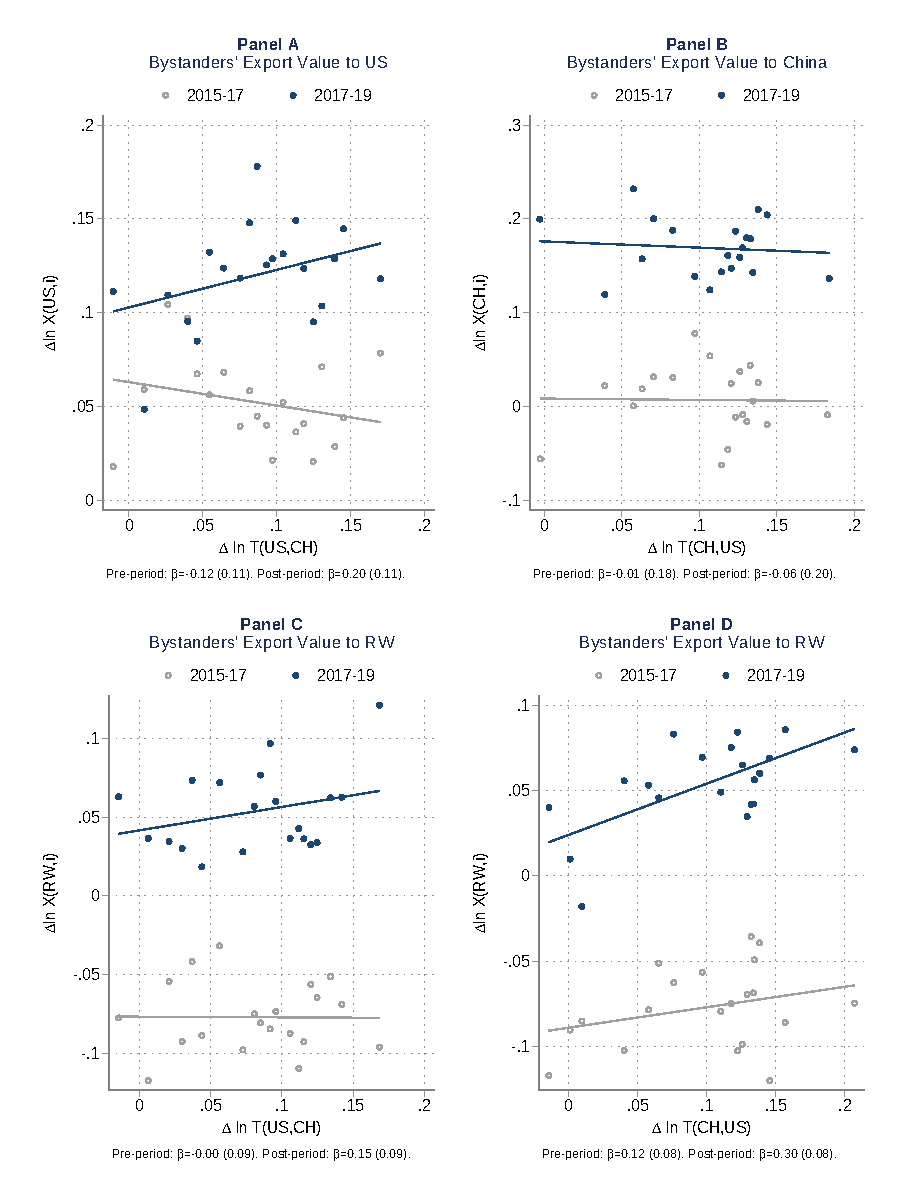
\includegraphics[width=\linewidth,height=\figh,keepaspectratio]{figures/paper/fig_a4_fe.pdf}
  \end{column}
  \begin{column}{0.335\textwidth}
    \centering
    \figlabel{Replication}
    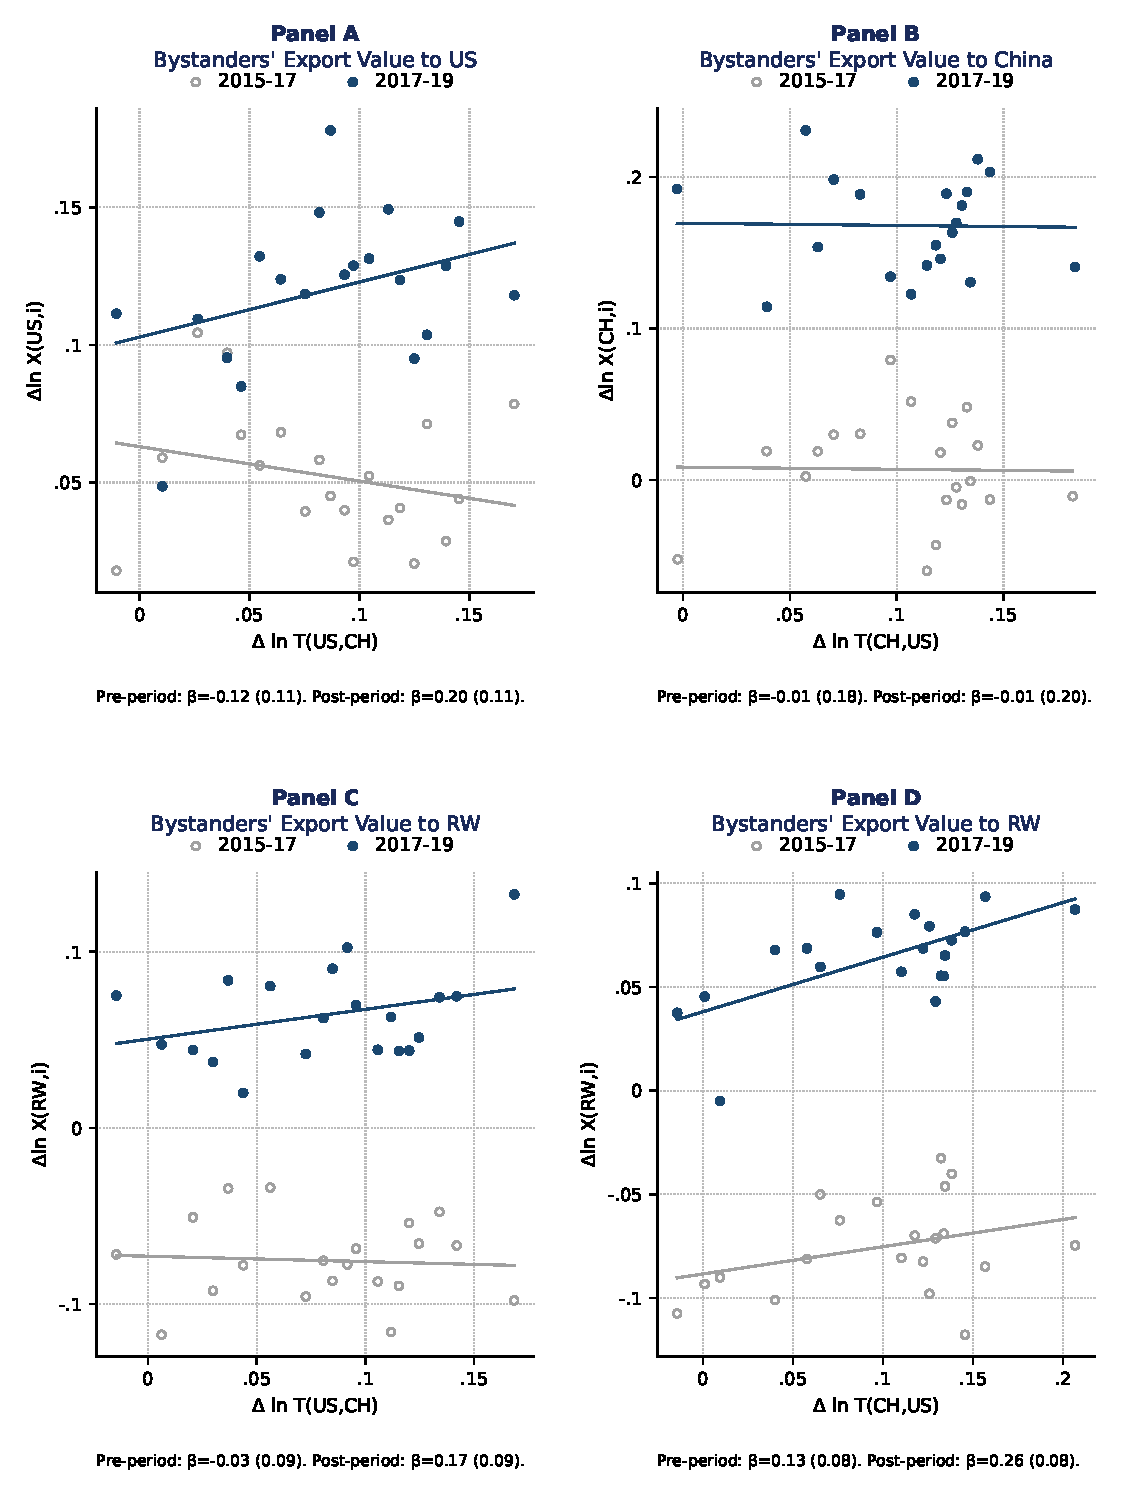
\includegraphics[width=\linewidth,height=\figh,keepaspectratio]{figures/replication/fig_a4_fe.pdf}
  \end{column}
  \begin{column}{0.28\textwidth}
    \slopes{Post-period slope, with FE}{%
      A\enspace US & \pv{0.20}{*} & \pv{0.20}{*} \\
      B\enspace CH & \pv{$-$0.06}{} & \pr{$-$0.01}{} \\
      C\enspace RW & \pv{0.15}{*} & \pr{0.17}{*} \\
      D\enspace RW & \pv{0.30}{***} & \pr{0.26}{***} \\}
    \vspace{0.5em}
    {\footnotesize\raggedright Same conclusions as Figure 1\par}
  \end{column}
\end{columns}
\note{\notehead{10. Robustness: exporter $\times$ sector fixed effects}{0:45}{6:20}
  Figure A.4 adds exporter-by-sector fixed effects. This compares products within the same country and sector, absorbing common growth differences, such as stronger growth across a country's machinery exports.
\\[0.6em]
  The table on the right shows the same qualitative pattern: positive responses into the US and the rest of the world, and no detectable average response into China.
\\[0.6em]
  The US slope falls to 0.20. The US response and the rest-of-world response to US tariffs are significant only at ten percent; the response to Chinese tariffs remains significant at one percent. My replication closely matches these results.}
\end{frame}

\begin{frame}{US--China bilateral trade (Fig.\ A.3)}
\begin{columns}[T,onlytextwidth]
  \begin{column}{0.485\textwidth}
    \centering
    \figlabel{Paper}
    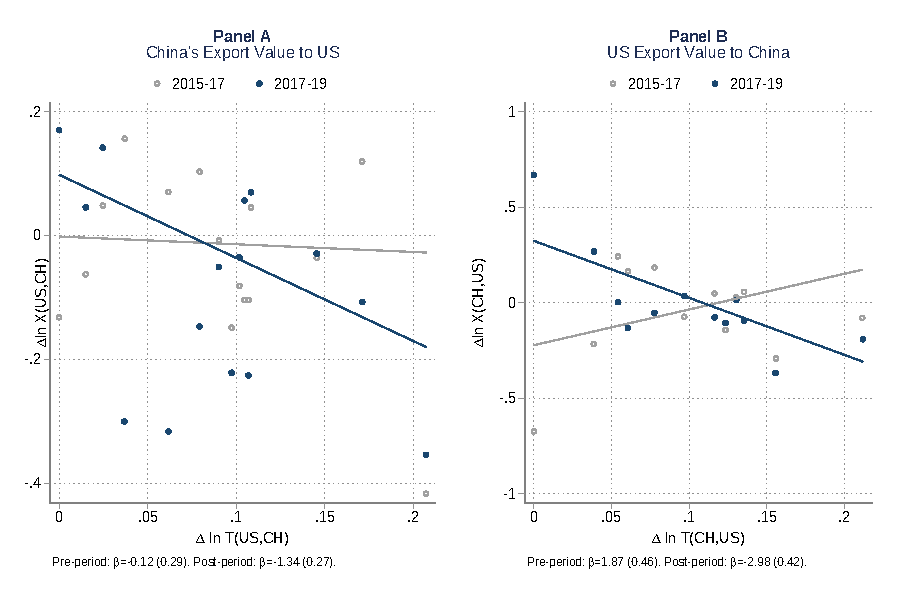
\includegraphics[width=\linewidth,height=3.5cm,keepaspectratio]{figures/paper/fig_a3_bilateral.pdf}
  \end{column}
  \begin{column}{0.485\textwidth}
    \centering
    \figlabel{Replication}
    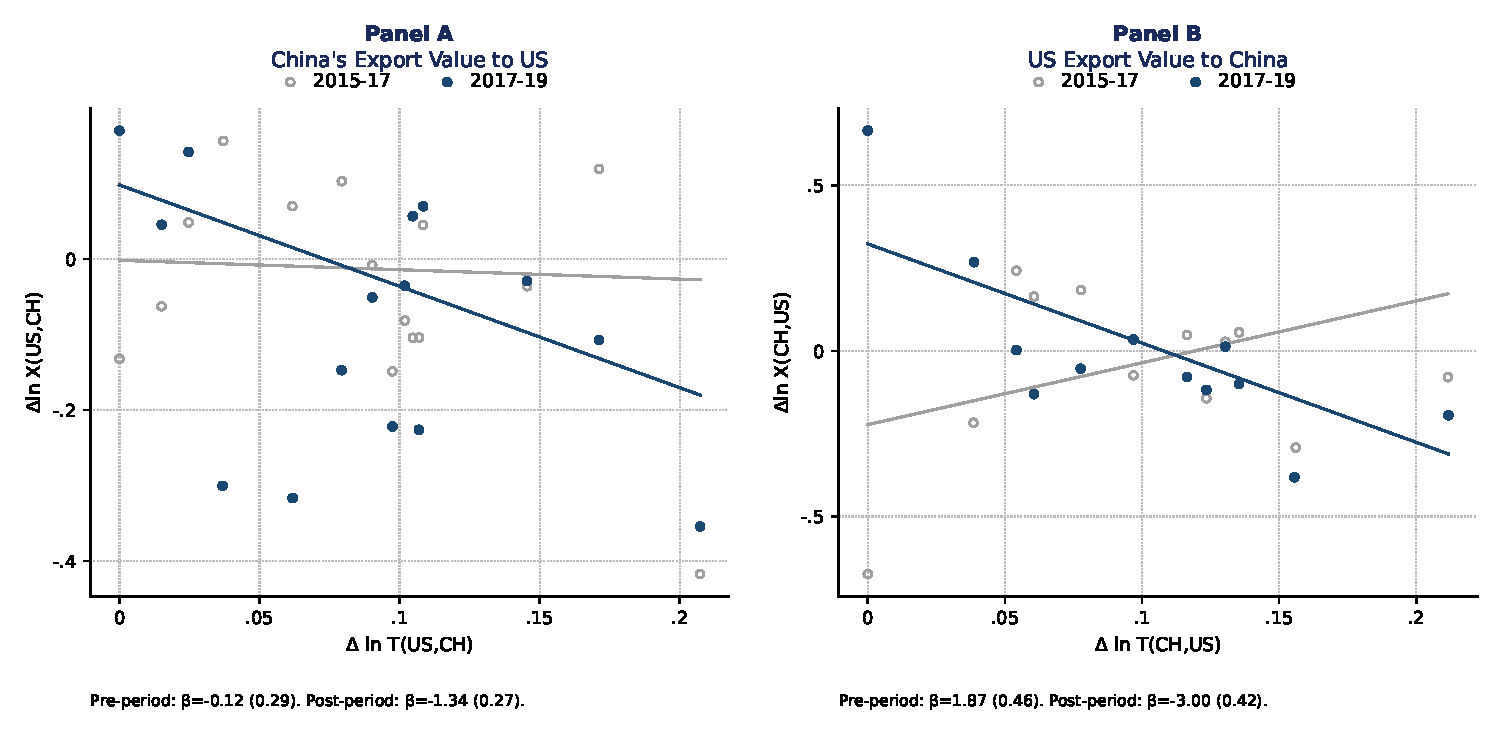
\includegraphics[width=\linewidth,height=3.5cm,keepaspectratio]{figures/replication/fig_a3_bilateral.pdf}
  \end{column}
\end{columns}
\framefill
\begin{itemize}\small
  \item Post-period slopes: China$\to$US $-1.34$ (0.27) in both;
        US$\to$China $-2.98$ (0.42) in the paper,
        \textcolor{PennRed}{$-3.00$} (0.42) here
  \item The tariffs cut US--China trade directly
\end{itemize}
\note{\notehead{11. US--China bilateral trade}{0:40}{7:00}
  Figure A.3 examines the directly targeted trade: China's exports to the US and US exports to China. The paper is on the left and the replication on the right.
\\[0.6em]
  Both war-period slopes are negative. China's response is minus 1.34 in both versions; the US response is minus 3.00 in mine, compared with minus 2.98 in the paper.
\\[0.6em]
  Thus, products facing larger tariffs had weaker bilateral export growth. The prewar patterns differ: China's slope is near zero, while the US slope is positive.}
\end{frame}

\begin{frame}{What the replicated results say}
\begin{itemize}
  \item Stronger relative export growth to the US ($\beta = 0.31$)
        and RW (0.22 and 0.25) in tariff-exposed products
  \item No detectable average response into China ($\beta = 0.05$, s.e.\ 0.19)
  \item Positive RW responses support expanded export opportunities
        across markets
\end{itemize}
\framefill
\begin{alertblock}{Pre-trends are somewhat stronger with today's data}
RW prewar slopes: $-0.16^{**}$ on US tariffs (paper $-0.14^{*}$) and
$0.13^{*}$ on Chinese tariffs (paper 0.11). The positive Chinese-tariff
pretrend qualifies the interpretation of the postwar response.
\end{alertblock}
\note{\notehead{12. What the replicated results say}{0:55}{7:55}
  The replicated results show stronger relative export growth to the US and the rest of the world in tariff-exposed products. The China estimate is 0.05 with a standard error of 0.19, so it is too imprecise to establish an average response.
\\[0.6em]
  Positive rest-of-world responses support expansion beyond trade diversion. These are comparisons across products, however, not estimates of the change in total world trade.
\\[0.6em]
  The red box highlights a qualification. The prewar rest-of-world slope against Chinese tariffs is 0.13 and significant at ten percent, so some later growth may continue an earlier trend. Against US tariffs, the prewar slope is minus 0.16. That raises a different concern about parallel trends, rather than showing the same positive trend continuing.}
\end{frame}

%%% ==================================================================
\section[3. Rest of the paper]{The rest of the paper}
%%% ==================================================================

\begin{frame}[c]{Outline}
\sectionoutline{3}
\note{\notehead{13. Outline: section 3}{0:05}{8:00}
  I'll briefly explain the paper's remaining findings, which I did not replicate.}
\end{frame}

\begin{frame}{The rest of the paper (not replicated)}
\begin{itemize}
  \item \textbf{Gains vary widely across countries} (Fig.~2): mean $+6.4\%$,
        s.d.\ 6.2 points; Thailand $+14.6\%$, Ukraine $-11.3\%$
  \item \textbf{Mostly from how each country responds} (Fig.~3):
        country-specific responses explain 76\% of the variation, sectors 24\%
  \item \textbf{Winners and losers} (Fig.~4): Thailand, Taiwan and the UK
        replace the taxed goods and expand in every market; Ukraine and
        Colombia lose sales everywhere
\end{itemize}
\note{\notehead{14. The rest of the paper}{1:00}{9:00}
  The rest of the paper makes three points.
\\[0.6em]
  First, predicted growth in targeted products relative to other products varies widely across countries. The average is 6.4 percent, with a standard deviation of 6.2 percentage points. Thailand's estimate is positive, at 14.6 percent; Ukraine's is negative, at minus 11.3 percent.
\\[0.6em]
  Second, country-specific tariff responses explain about seventy-six percent of the variation. Sector-specific responses explain about twenty-four percent. Countries' initial export baskets alone explain much less.
\\[0.6em]
  Third, the model links these differences to demand and supply. Thailand, Taiwan, and the UK substitute for US and Chinese goods. Expansion can lower their costs and support exports elsewhere. Ukraine and Colombia complement those goods: weaker demand reduces scale and can raise costs. These mechanisms are inferred through the model.}
\end{frame}

%%% ==================================================================
\section[4. Takeaways]{Takeaways}
%%% ==================================================================

\begin{frame}[c]{Outline}
\sectionoutline{4}
\note{\notehead{15. Outline: section 4}{0:05}{9:05}
  I'll close with the main findings and limitations.}
\end{frame}

\begin{frame}{Takeaways}
\begin{itemize}
  \item \textbf{Replication:} all 20 regressions match on the authors' data;
        rebuilt-data coefficients differ by at most 0.05
  \item \textbf{Result:} stronger relative export growth to the US and RW
        in tariff-exposed products
  \item \textbf{Rest of the paper:} large cross-country differences, from
        country-specific elasticities
\end{itemize}
\framefill
\begin{alertblock}{Limitations}
The rebuild uses a newer Comtrade vintage; US Census inputs come from
the authors' package; the main model (Figures 2--4) is not replicated.
\end{alertblock}
\note{\notehead{16. Takeaways}{0:45}{9:50}
  Using the authors' processed data, my Python code matches all twenty regressions at the reported precision. Rebuilding the datasets with fresh Comtrade data produces coefficient differences of at most 0.05.
\\[0.6em]
  The central pattern remains: stronger relative export growth to the US and the rest of the world in tariff-exposed products, although prewar trends qualify the causal interpretation.
\\[0.6em]
  The paper also finds substantial country differences. My replication covers the average responses, not the model behind Figures 2 through 4. It uses a newer Comtrade vintage and relies on Census inputs supplied in the authors' package.}
\end{frame}

\begin{frame}[c]{Thank you!}
\centering
{\large\emph{The US--China Trade War and Global Reallocations}\par}
\vspace{0.4em}
A replication\par
\vspace{1.2em}
Apostolos Kyratzis\par
\vspace{0.3em}
{\footnotesize Code, selected data, and download instructions:\par
\href{https://github.com/akyratzis/STAT-5200---Applied-Econometrics-I/tree/main/Replication\%20Study}%
  {\texttt{github.com/akyratzis/STAT-5200-{}-{}-Applied-Econometrics-I/tree/main/Replication~Study}}\par}
\note{\notehead{17. Thank you}{0:10}{10:00}
  Thank you. The GitHub link provides the code, documentation, selected data, and instructions for downloading the remaining inputs.}
\end{frame}

\end{document}
